%                      Code_Saturne version 1.3
%                      ------------------------
%
%     This file is part of the Code_Saturne Kernel, element of the
%     Code_Saturne CFD tool.
% 
%     Copyright (C) 1998-2007 EDF S.A., France
%
%     contact: saturne-support@edf.fr
% 
%     The Code_Saturne Kernel is free software; you can redistribute it
%     and/or modify it under the terms of the GNU General Public License
%     as published by the Free Software Foundation; either version 2 of
%     the License, or (at your option) any later version.
% 
%     The Code_Saturne Kernel is distributed in the hope that it will be
%     useful, but WITHOUT ANY WARRANTY; without even the implied warranty
%     of MERCHANTABILITY or FITNESS FOR A PARTICULAR PURPOSE.  See the
%     GNU General Public License for more details.
% 
%     You should have received a copy of the GNU General Public License
%     along with the Code_Saturne Kernel; if not, write to the
%     Free Software Foundation, Inc.,
%     51 Franklin St, Fifth Floor,
%     Boston, MA  02110-1301  USA
%
%-----------------------------------------------------------------------
\section{SOLUTION FOR CASE 1}
The first thing to do before running \CS\ is to prepare the computation
directories. In this first example, the study directory ``T\_JUNCTION'' will be
created, containing a single calculation directory CAS1. This is done by typing
the command {\itshape cree\_sat -etude T\_JUNCTION CAS1}.

The mesh files should be copied in the directory MAILLAGE.

The \CS\ Graphical Interface is launched by typing the command
{\itshape ./SaturneGUI} in the DATA subdirectory of the CAS1 directory.
The following graphic window opens (fig \ref{fig1_e1}).  

\begin{figure}[ht]
\begin{center}
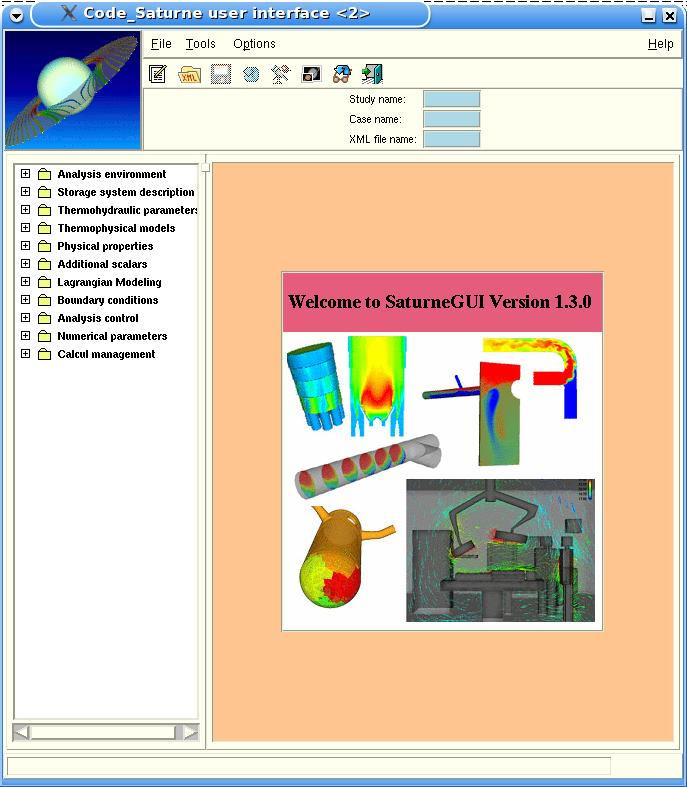
\includegraphics[width=12cm]{\repgraphics/c1_capture01.jpg} 
\caption{User interface}
\label{fig1_e1}
\end{center}
\end{figure}


\clearpage
Go to the {\itshape File} menu and click on {\itshape New file} to open a new
calculation data file, as shown in the figure
\ref{fig2_e1}. 

\begin{figure}[ht]
\begin{center}
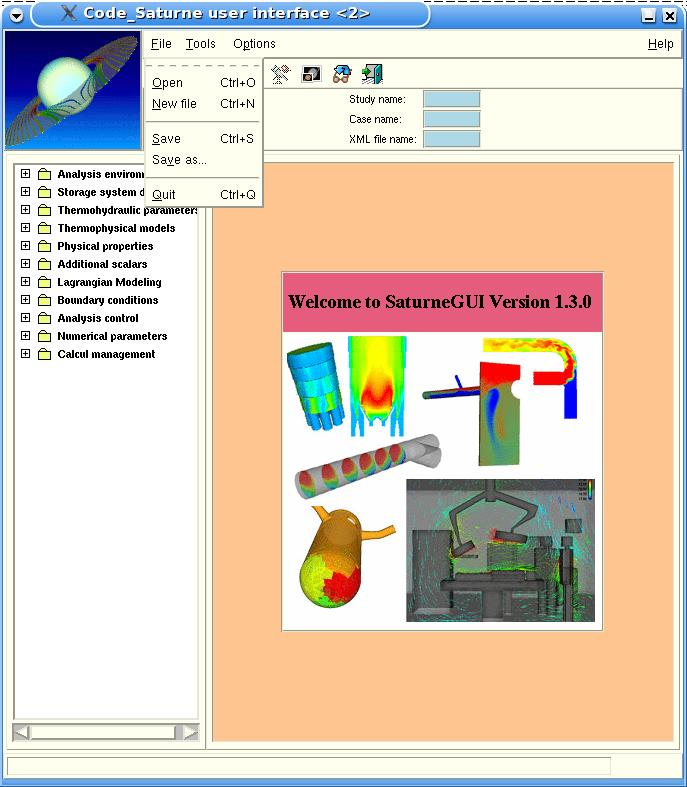
\includegraphics[width=12cm]{\repgraphics/c1_capture02.jpg} 
\caption{Opening a new file}
\label{fig2_e1}
\end{center}
\end{figure}


\clearpage
The interface automatically updates the following information: 
\begin{itemize}
	\item Study name
	\item Case name
	\item Directory of the case
	\item Associated sub-directories of the case
\end{itemize}

\begin{figure}[ht]
\begin{center}
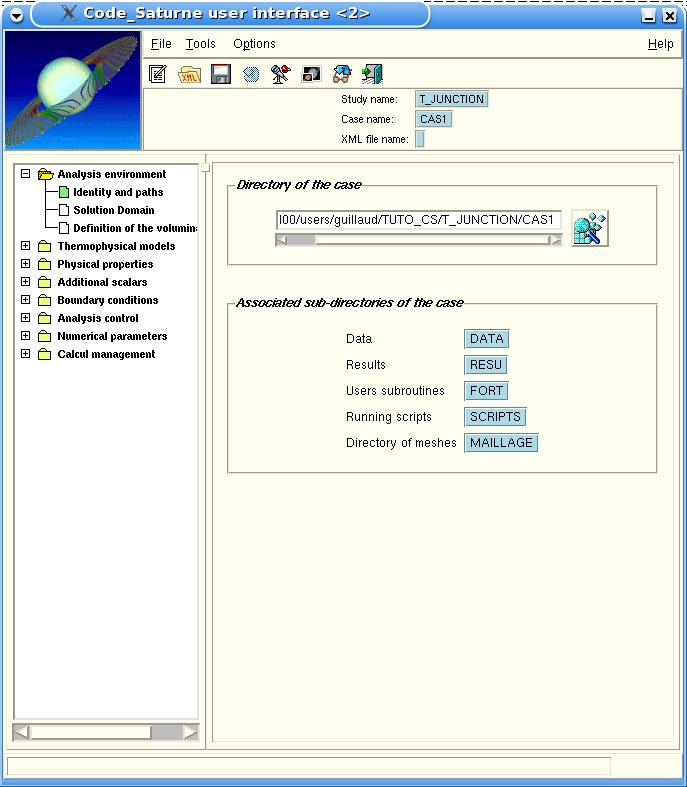
\includegraphics[width=12cm]{\repgraphics/c1_capture03.jpg} 
\caption{Identity and paths}
\label{fig3_e1}
\end{center}
\end{figure}


\clearpage
Save the case to give a name to the new {\itshape XML file} by opening the
{\itshape File} menu and clicking on {\itshape Save as...}. A new window will
appear, enter the name of the case in {\itshape File Name} then click on
{\itshape Save}.

Remember to save the case regularly throughout the preparation of the calculation.

\begin{figure}[ht]
\begin{center}
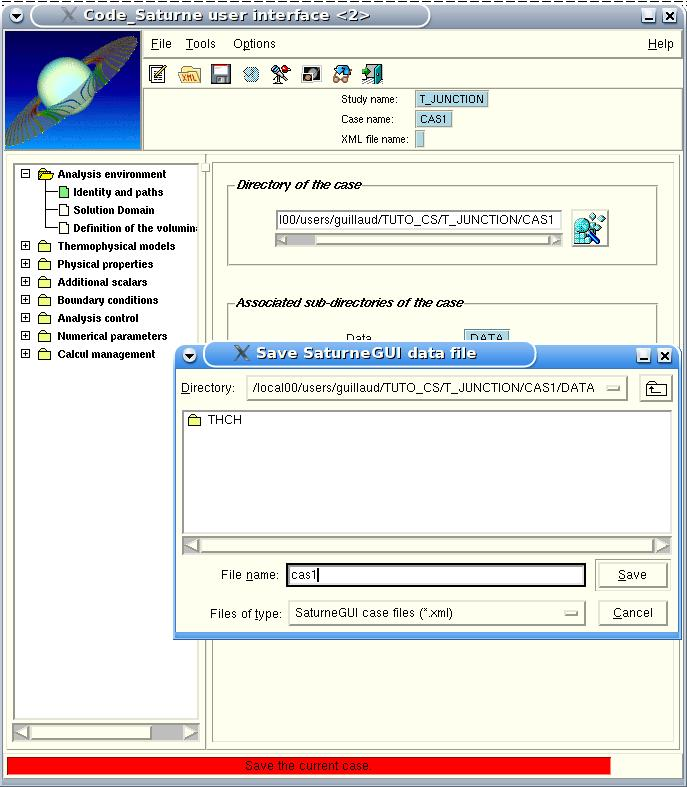
\includegraphics[width=12cm]{\repgraphics/c1_capture04.jpg} 
\caption{Saving the {\itshape XML} file}
\label{fig4_e1}
\end{center}
\end{figure}


\clearpage
The next step is to specify the mesh(es) to be used for the calculation.
Click on the item {\itshape Solution Domain} 
under the heading {\itshape Analysis environment}. The list of all
meshes available in the folder {\itshape MAILLAGE} appears in the
window {\itshape List of meshes}. Delete the mesh(es) you will not
use\footnote{this operation only deletes the selected entries from the list, it
does not delete the mesh file in the MAILLAGE directory}. In this case only the
mesh {\itshape downcomer.des} is needed. 

\begin{figure}[ht]
\begin{center}
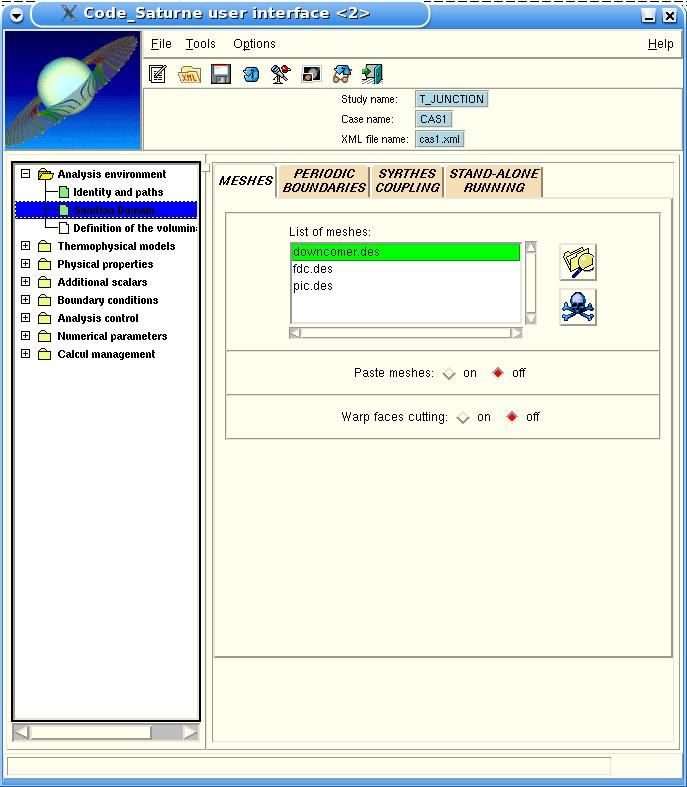
\includegraphics[width=12cm]{\repgraphics/c1_capture05.jpg} 
\caption{Meshes: list of meshes}
\label{fig5_e1}
\end{center}
\end{figure}

On this item ({\itshape Solution Domain}) there are three other tabs: 
\begin{itemize}
	\item PERIODIC BOUNDARIES
	\item SYRTHES COUPLING
	\item STAND-ALONES RUNNING
\end{itemize}
They are not used in this case. Keep the default values.

\clearpage
The item {\itshape Analysis features} under the heading {\itshape Thermophysical
environment} allows to define the type of flow to be simulated. In this case, a
steady flow will be chosen.  

\begin{figure}[ht]
\begin{center}
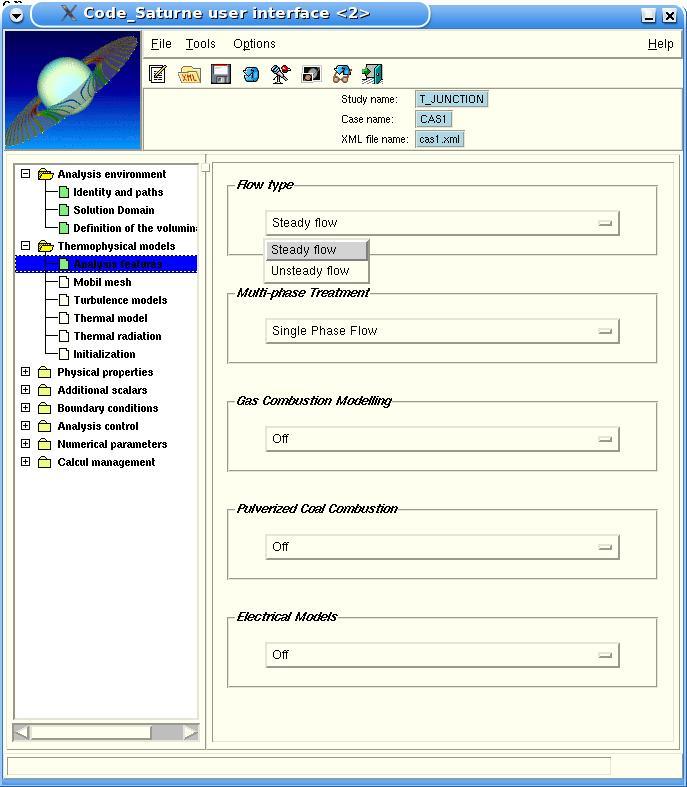
\includegraphics[width=12cm]{\repgraphics/c1_capture07.jpg} 
\caption{Flow type}
\label{fig7_e1}
\end{center}
\end{figure}


\clearpage
The turbulence model is selected in the following list:\\
\hspace*{1cm}$\bullet\ $laminar flow (no model)\\
\hspace*{1cm}$\bullet\ $mixing length\\
\hspace*{1cm}$\bullet\ $k-$\varepsilon$\\
\hspace*{1cm}$\bullet\ $k-$\varepsilon$ Linear Production\\
\hspace*{1cm}$\bullet\ $Rij-$\varepsilon$ LLR\\
\hspace*{1cm}$\bullet\ $Rij-$\varepsilon$ SSG\\
\hspace*{1cm}$\bullet\ $v2f ($\varphi$ model)\\
\hspace*{1cm}$\bullet\ $k-$\omega$ SST\\
\hspace*{1cm}$\bullet\ $LES (Smagorinsky)\\
\hspace*{1cm}$\bullet\ $LES (dynamic model)

\begin{figure}[ht]
\begin{center}
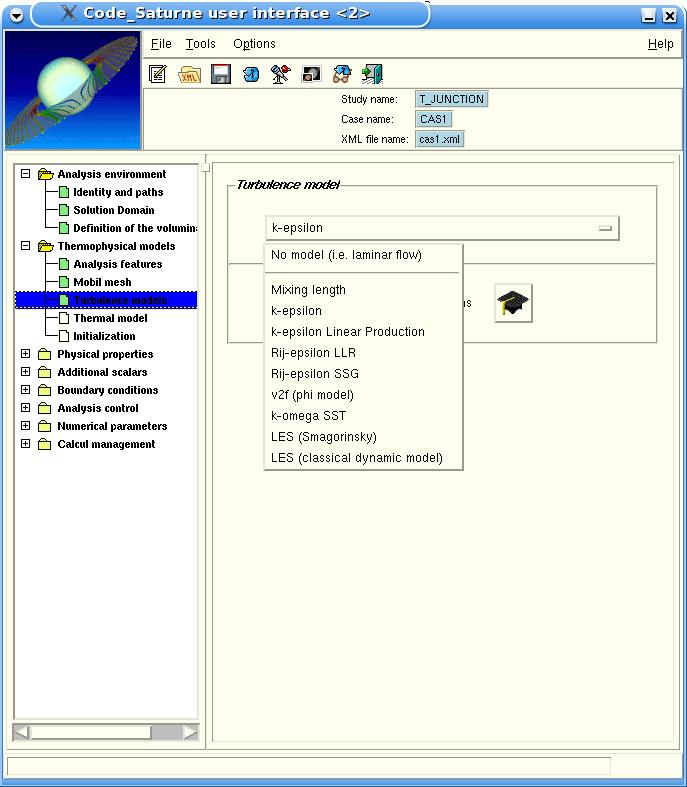
\includegraphics[width=12cm]{\repgraphics/c1_capture09.jpg} 
\caption{Turbulence model: list of models}
\label{fig9_e1}
\end{center}
\end{figure}


\clearpage
In this case, the k-$\varepsilon$ model is used.

\begin{figure}[ht]
\begin{center}
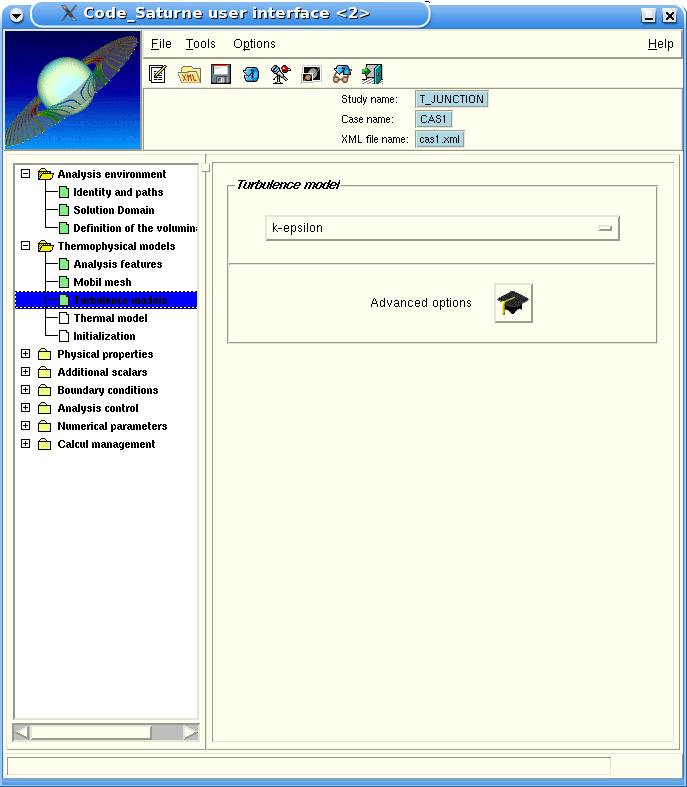
\includegraphics[width=12cm]{\repgraphics/c1_capture10.jpg} 
\caption{Turbulence model: choice of a model}
\label{fig10_e1}
\end{center}
\end{figure}


\clearpage
For this study the equation for temperature must be solved. Click on the item
{\itshape Thermal model} to
choose between:\\
\hspace*{1cm}$\bullet\ $No thermal scalar\\
\hspace*{1cm}$\bullet\ $Temperature (Celsius degrees)\\
\hspace*{1cm}$\bullet\ $Temperature (Kelvin)\\
\hspace*{1cm}$\bullet\ $Enthalpy

\begin{figure}[ht]
\begin{center}
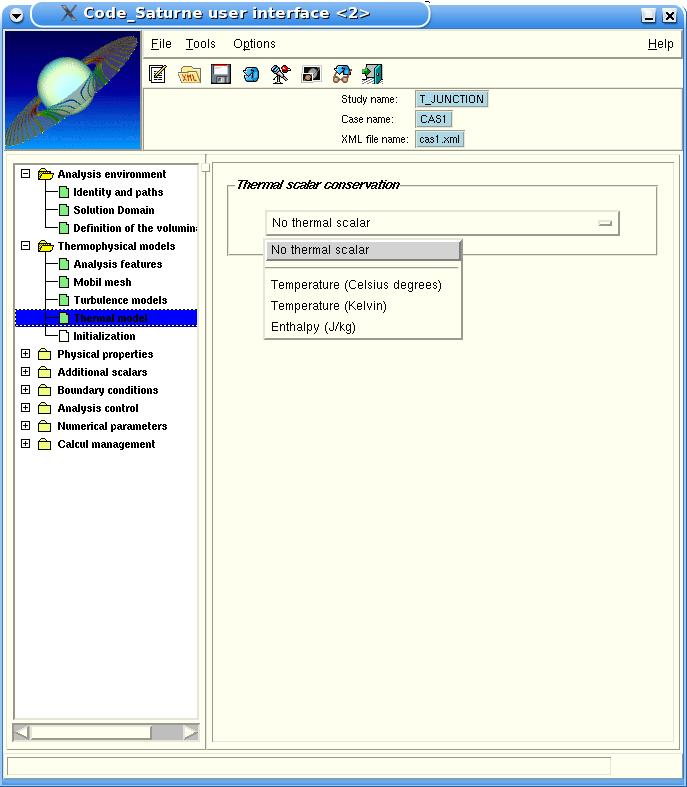
\includegraphics[width=12cm]{\repgraphics/c1_capture11.jpg} 
\caption{Thermal scalar conservation: list of models}
\label{fig11_e1}
\end{center}
\end{figure}


\clearpage
In the present case, select {\itshape Temperature (Celsius degrees)}.
\begin{figure}[ht]
\begin{center}
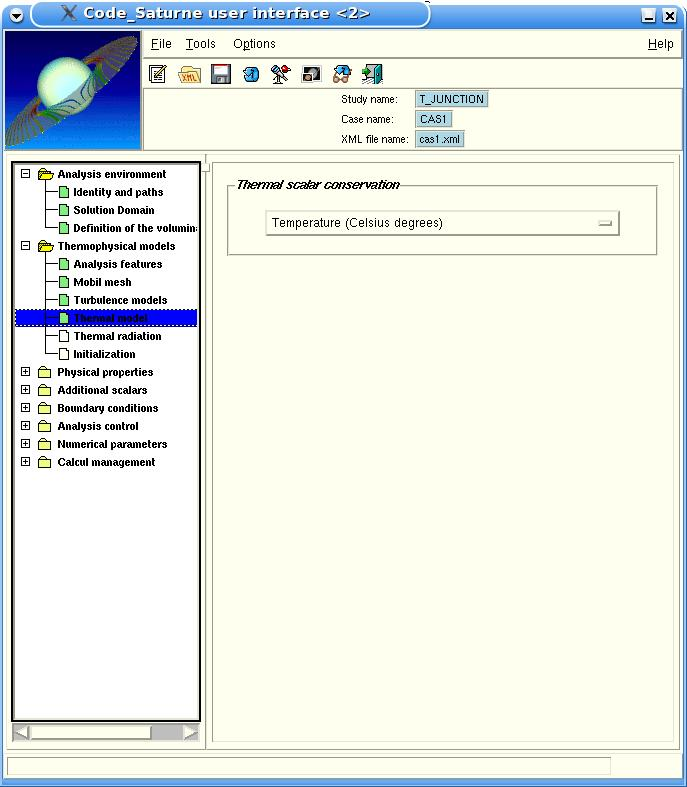
\includegraphics[width=12cm]{\repgraphics/c1_capture12.jpg} 
\caption{Thermal scalar conservation: choice of a model}
\label{fig12_e1}
\end{center}
\end{figure}

There are no radiative transfers in our case, so the item is ignored.

\clearpage
To initialize variables at the instant $t=0\ s$, go to the item {\itshape Initialization}. 
Here the velocity, the thermal scalar and the turbulence can be initialized. In
this case, the default values can be kept: zero velocity, an initial temperature
of 20\degresC\ and a turbulence level based on a reference velocity of $1\
m.s^{-1}$. Specific zones can be defined with different initializations. In this
case, only the default ``all cells'' is used.

\begin{figure}[ht]
\begin{center}
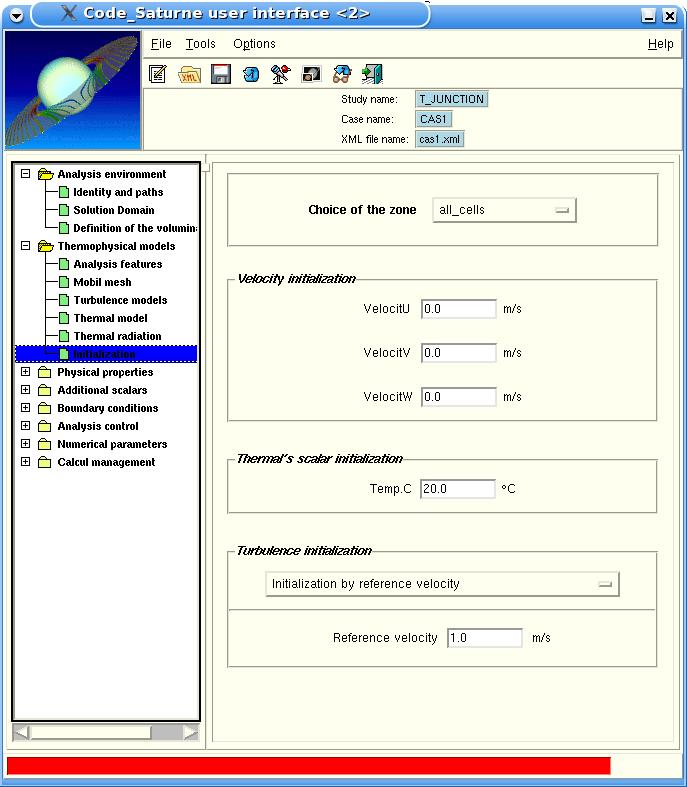
\includegraphics[width=12cm]{\repgraphics/c1_capture14.jpg} 
\caption{Initialization of dynamic variables}
\label{fig14_e1}
\end{center}
\end{figure}


\clearpage
The initial value for the thermal scalar also appears in the item
{\itshape Definition and Initialization} under the heading
{\itshape Additional scalars}, where more options concerning the scalars can be
specified. The value of the initial value can be modified in any of the two
pages. But in case there are additional scalars ({\em i.e.} other than the
thermal scalar), their initialization is only possible in the {\itshape
Additional scalars} page.

\begin{figure}[ht]
\begin{center}
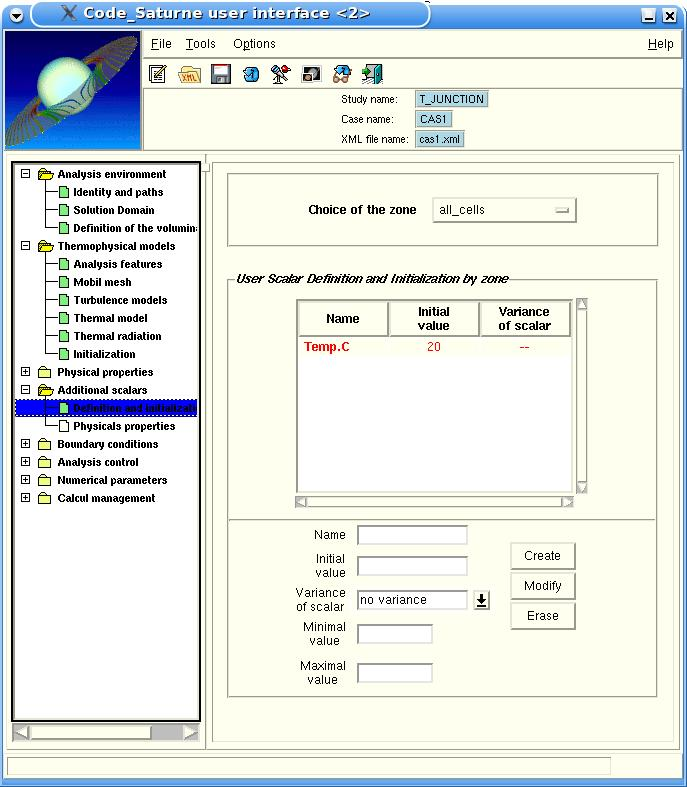
\includegraphics[width=12cm]{\repgraphics/c1_capture15.jpg} 
\caption{Initialization of the scalar}
\label{fig15_e1}
\end{center}
\end{figure}


\clearpage
Click on the thermal scalar in the list, to change: 
\begin{itemize}
	\item its name
	\item its initial value
	\item its minimal value
	\item its maximal value
\end{itemize}
In this case the temperature can vary between 0\degresC\ and 400\degresC.
After entering the new values, click on {\itshape Modify} in order to validate
these changes.

\begin{figure}[ht]
\begin{center}
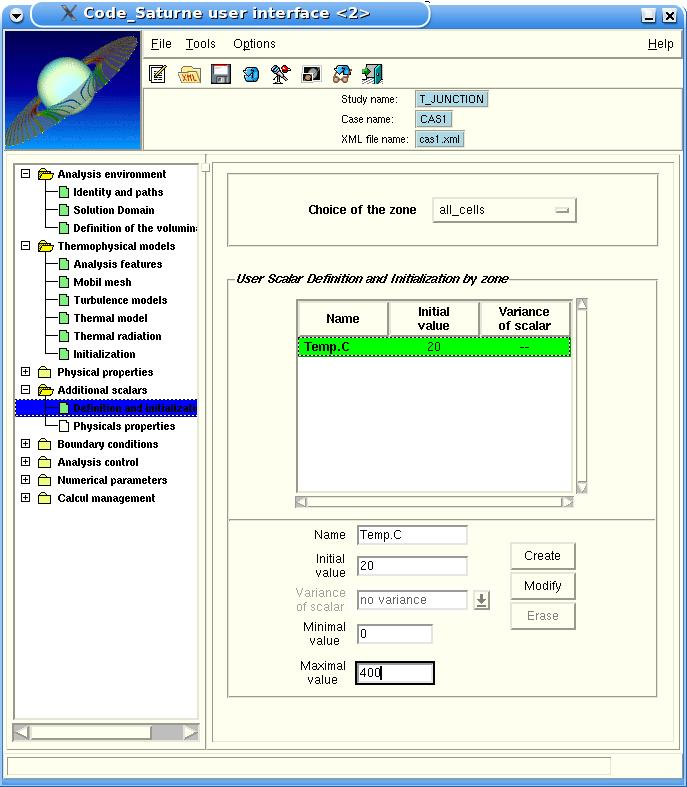
\includegraphics[width=12cm]{\repgraphics/c1_capture16.jpg} 
\caption{Initialization of the scalar}
\label{fig16_e1}
\end{center}
\end{figure}

The item {\itshape Physicals properties} under the heading {\itshape Additional
scalars}\footnote{not to be confused with the heading {\itshape Physical
properties} in the main list} is used to specify the physical properties
of the additional scalars, {\em i.e.} those that are not the thermal scalar. In
this case there are no additional scalars, the item is therefore unused.


\clearpage
Under the heading {\itshape Physical properties} in the main list,
the item {\itshape Reference values} allows to set the reference pressure.
Use the default value of $101\,300\ Pa$. 

\begin{figure}[ht]
\begin{center}
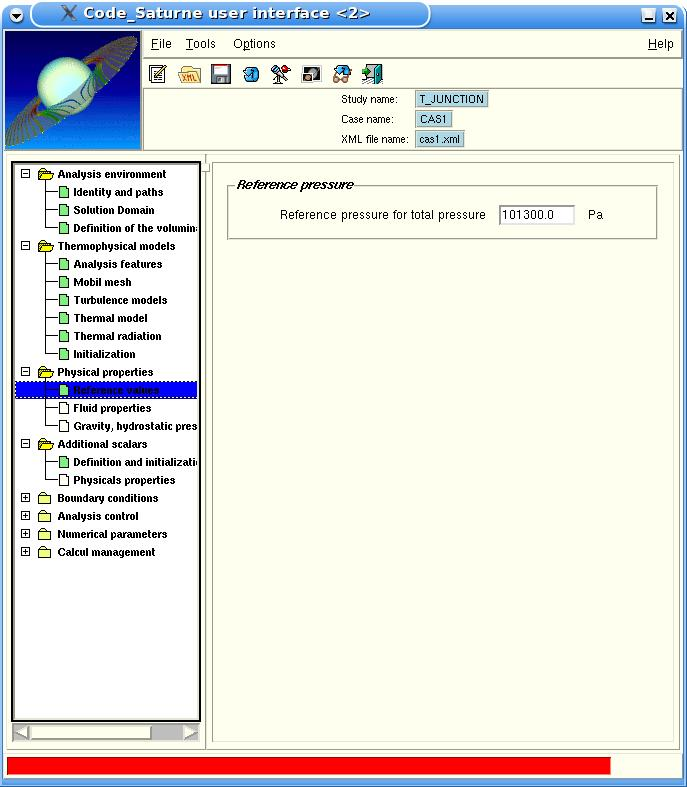
\includegraphics[width=12cm]{\repgraphics/c1_capture17.jpg} 
\caption{Physical properties: reference pressure}
\label{fig17_e1}
\end{center}
\end{figure}


\clearpage
Specify the fluid physical characteristics in the item {\itshape Fluid
properties}: 
\begin{itemize}
	\item Density
	\item Viscosity
	\item Specific Heat
	\item Thermal Conductivity
\end{itemize}

In this case they are all constant.
\begin{itemize}
	\item Density $ = 725.735\ kg.m^{-3}$ 
	\item Viscosity $ = 0.895\times 10^{-4}\ kg.m^{-1}.s^{-1}$
	\item Specific Heat $  = 5\,483\ J.kg^{-1}.\mbox{\degresC}^{-1}$ 
	\item Thermal Conductivity $ = 0.02495\ W.m^{-1}.K^{-1}$
\end{itemize}

\begin{figure}[ht]
\begin{center}
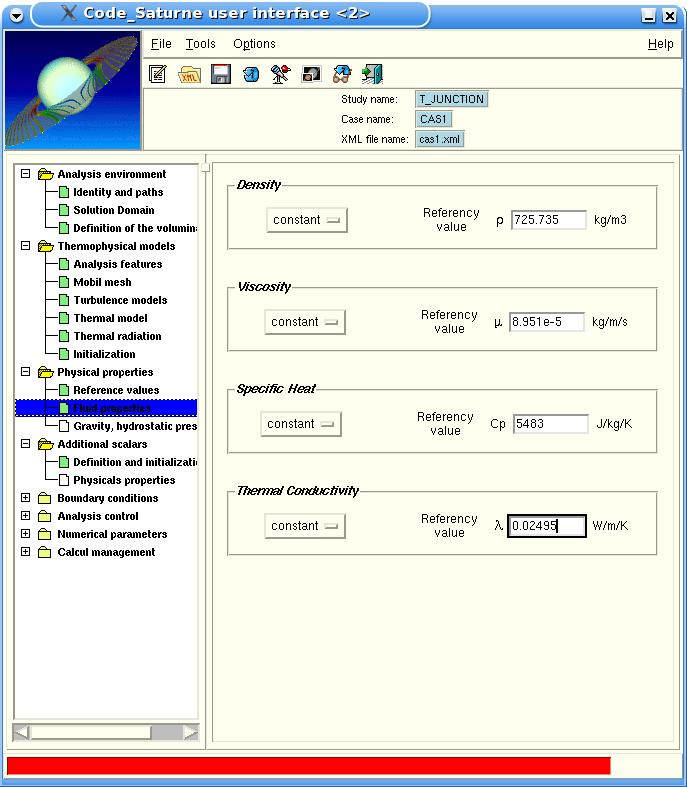
\includegraphics[width=12cm]{\repgraphics/c1_capture18.jpg} 
\caption{Physical properties: fluid properties}
\label{fig18_e1}
\end{center}
\end{figure}


\clearpage
Set the three components of gravity in the
{\itshape Gravity, hydrostatic pressure} item. 
In this case, since the gravity doesn't have
any influence on the flow, gravity can be set to 0.
As for the pressure interpolation interpolation method, keep the standard
default value. 

\begin{figure}[ht]
\begin{center}
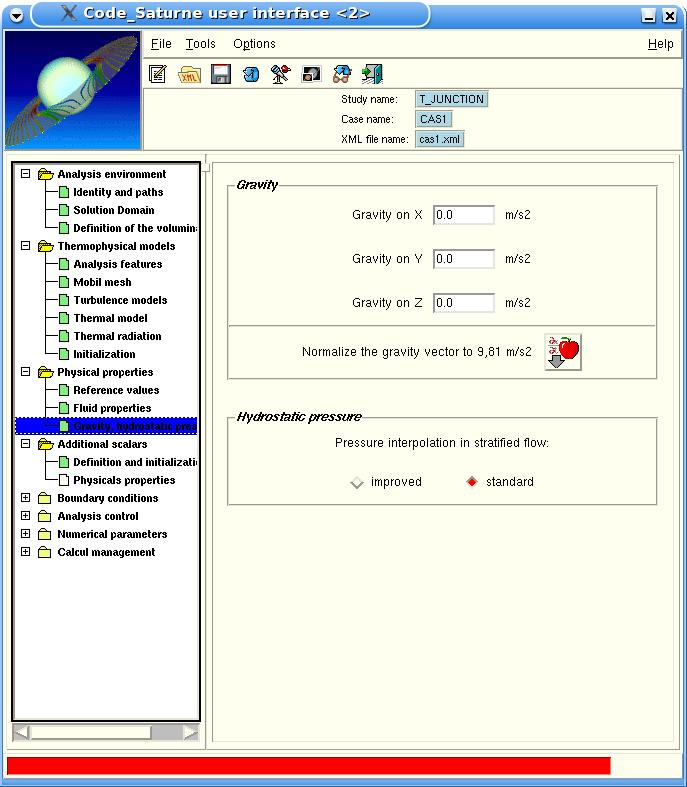
\includegraphics[width=12cm]{\repgraphics/c1_capture19.jpg} 
\caption{Physical properties: gravity, hydrostatic pressure}
\label{fig19_e1}
\end{center}
\end{figure}


\clearpage
Boundary conditions now need to be defined. Go to the item {\itshape Define
boundary regions} under the heading {\itshape Boundary conditions}.
The following window opens (fig \ref{fig20_e1}).  

\begin{figure}[ht]
\begin{center}
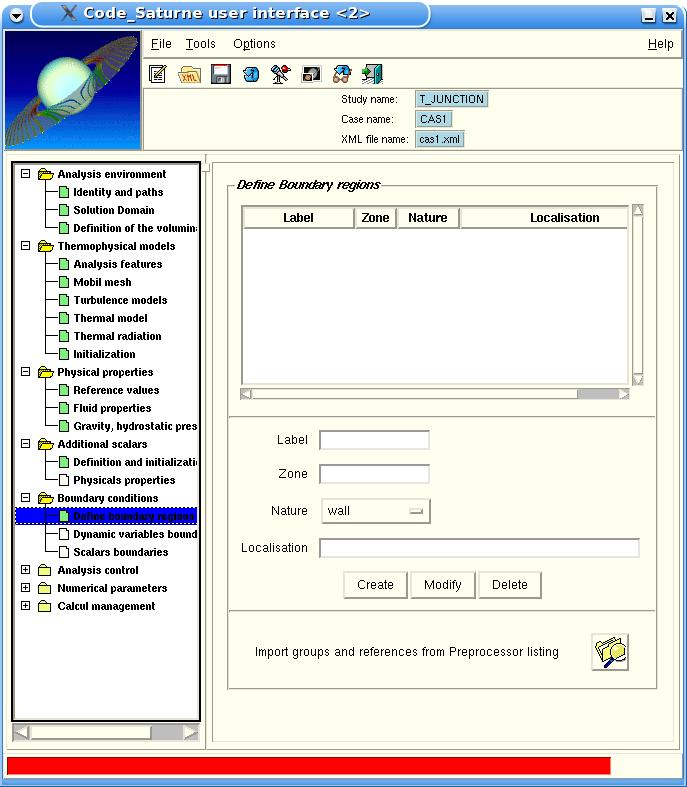
\includegraphics[width=12cm]{\repgraphics/c1_capture20.jpg} 
\caption{Creation of a boundary region}
\label{fig20_e1}
\end{center}
\end{figure}


\clearpage
Each boundary must be defined. The boundary faces will be grouped in
user-defined zones, based on their color or on geometrical conditions. For each
zone, a reference number, a label, a nature and a localization condition must be
assigned.
The different natures that can be assigned are:\\
\hspace*{1cm}$\bullet\ $wall\\
\hspace*{1cm}$\bullet\ $inlet\\
\hspace*{1cm}$\bullet\ $symmetry\\
\hspace*{1cm}$\bullet\ $outlet

The {\itshape Label} can be any character string. It is used to identify the
zone more easily. It usually corresponds to the nature of the zone.

The {\itshape Zone} number can be any integer. It will be used by the code to
identify the zone. No specific order or continuity in the numbering is needed.

The {\itshape Localization} is used to define the faces that belong to the
zone. It can be a color number, a group reference, geometrical conditions, on a
combination of them, related by ``or'' or ``and'' keywords.

\begin{figure}[ht]
\begin{center}
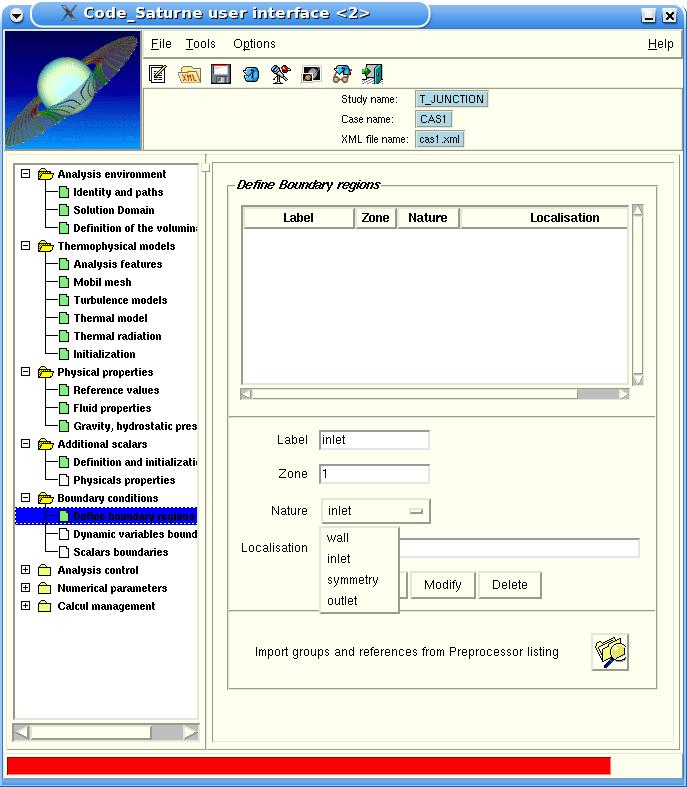
\includegraphics[width=12cm]{\repgraphics/c1_capture21.jpg} 
\caption{Creation of a boundary region}
\label{fig21_e1}
\end{center}
\end{figure}


\clearpage
The specification of the inlet condition is detailled in the following
pages. The settings will be as follows:\\
\hspace*{1cm}$\bullet\ ${\itshape Label}: inlet\\
\hspace*{1cm}$\bullet\ ${\itshape Zone}: 1\\
\hspace*{1cm}$\bullet\ ${\itshape Nature}: inlet\\
\hspace*{1cm}$\bullet\ ${\itshape Localization}: 1

\begin{figure}[ht]
\begin{center}
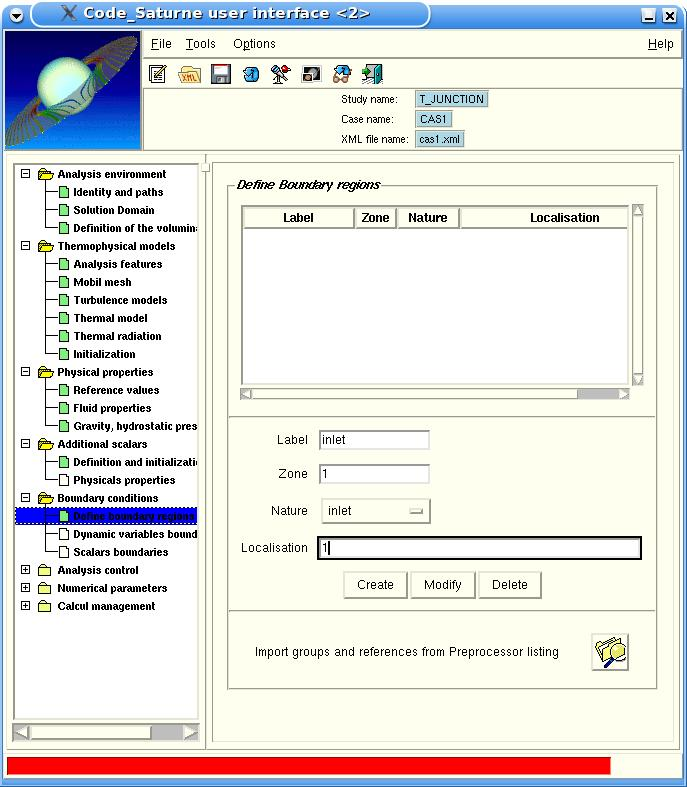
\includegraphics[width=12cm]{\repgraphics/c1_capture22.jpg} 
\caption{Creation of a boundary region: inlet region}
\label{fig22_e1}
\end{center}
\end{figure}



\clearpage
After typing all the information, click on {\itshape Create} to
create the boundary zone. It appears in the
{\itshape Define Boundary regions} list above.

\begin{figure}[ht]
\begin{center}
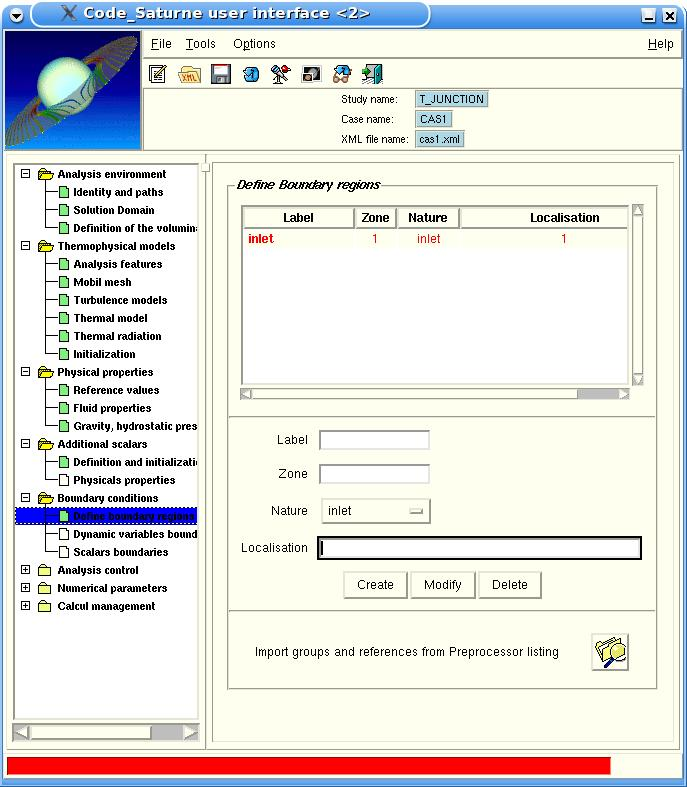
\includegraphics[width=12cm]{\repgraphics/c1_capture23.jpg} 
\caption{Creation of a boundary region: inlet region}
\label{fig23_e1}
\end{center}
\end{figure}

Remember to save the Xml file regularly!


\clearpage
Do the same thing for the other boundaries.

In our case, colors 8 and 9 are symmetry boundaries. One option can be to define
a separate zone for each color, as follows:
\begin{center}
\begin{tabular}{lcp{2cm}c}
Label & symmetry\_1 & & symmetry\_2 \\
Zone & 3 & & 4 \\
Nature & symmetry & & symmetry \\
Localization & 8 & & 9 \\
\end{tabular}
\end{center}

But it is usually faster to regroup the different colors in one single zone, as
shown on figure \ref{fig24_e1}. In our case, the localization for this zone is
the string ``8 or 9''.

\begin{figure}[ht]
\begin{center}
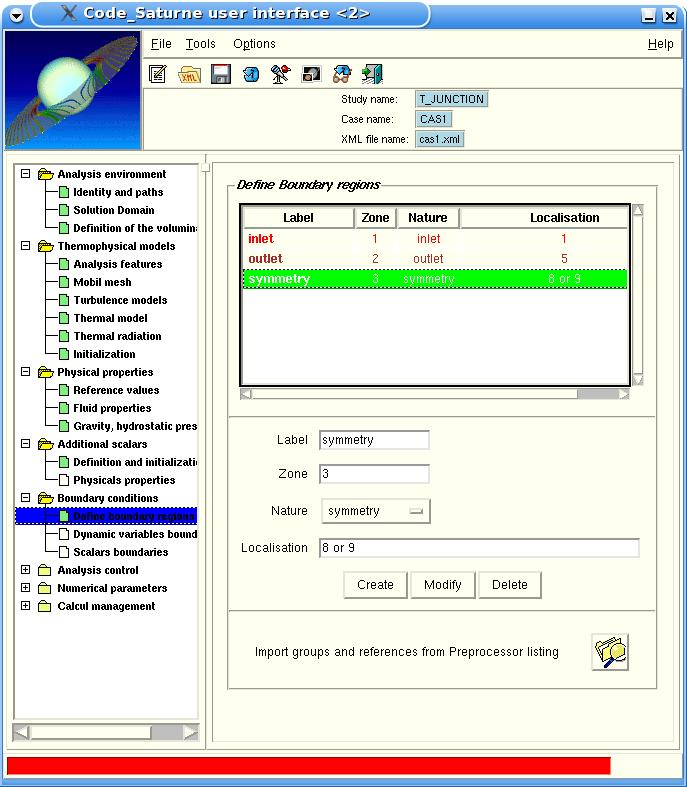
\includegraphics[width=12cm]{\repgraphics/c1_capture24.jpg} 
\caption{Creation of boundary regions: symmetry region}
\label{fig24_e1}
\end{center}
\end{figure}


\clearpage
The same treatment must be done for the wall conditions. All colors 2, 3, 4, 6
and 7 can be grouped in a single boundary zone.

After defining all the boundary zones, the Interface window will look as in
figure \ref{fig25_e1}.

\begin{figure}[ht]
\begin{center}
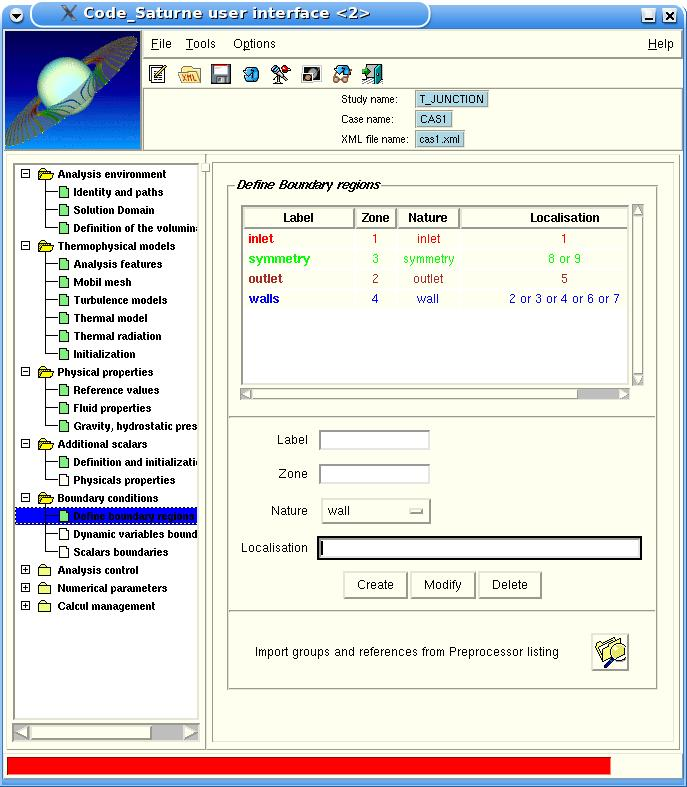
\includegraphics[width=12cm]{\repgraphics/c1_capture25.jpg} 
\caption{Creation of boundary regions}
\label{fig25_e1}
\end{center}
\end{figure}


\clearpage
Now that the boundary zones are defined, the boundary conditions assigned to
them will be specified. Click on the item
{\itshape Dynamic variables boundary} to set the boundary conditions for
velocity and turbulence. As shown on figure \ref{fig26_e1}, only the inlet and
wall boundary zones appear in the window. Indeed, symmetry and outlet conditions
do not need any user-defined data.

\begin{figure}[ht]
\begin{center}
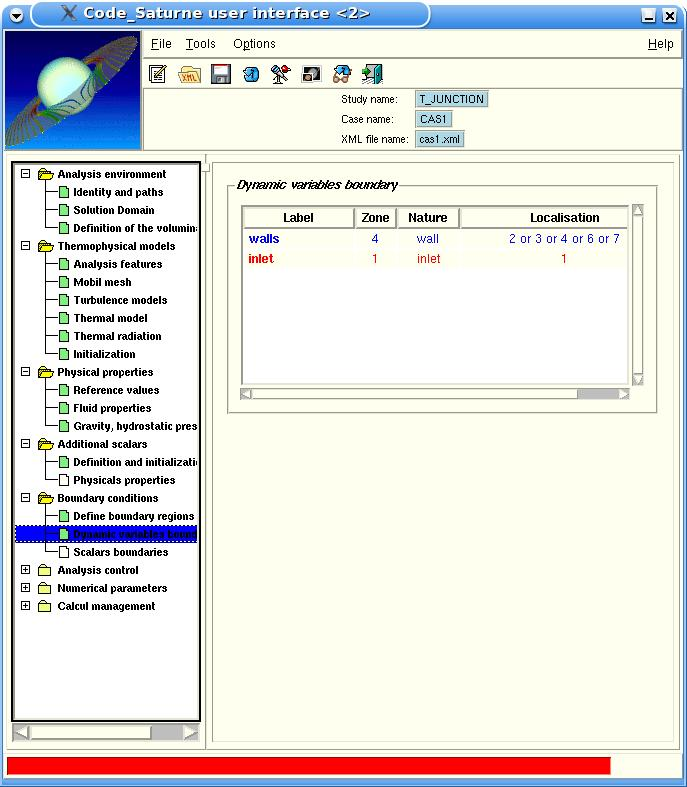
\includegraphics[width=12cm]{\repgraphics/c1_capture26.jpg} 
\caption{Dynamic variables boundary conditions}
\label{fig26_e1}
\end{center}
\end{figure}


\clearpage
Click on the label {\itshape inlet}. Enter the three components of the inlet
velocity. For the turbulence, chose the inlet condition based on a hydraulic
diameter and specify it.\\
\hspace*{1cm}$\bullet\ U = 1\ m.s^{-1}$\\
\hspace*{1cm}$\bullet\ V = 0\ m.s^{-1}$\\
\hspace*{1cm}$\bullet\ W = 0\ m.s^{-1}$\\
\hspace*{1cm}$\bullet\ D = 0.5\ m$

\begin{figure}[ht]
\begin{center}
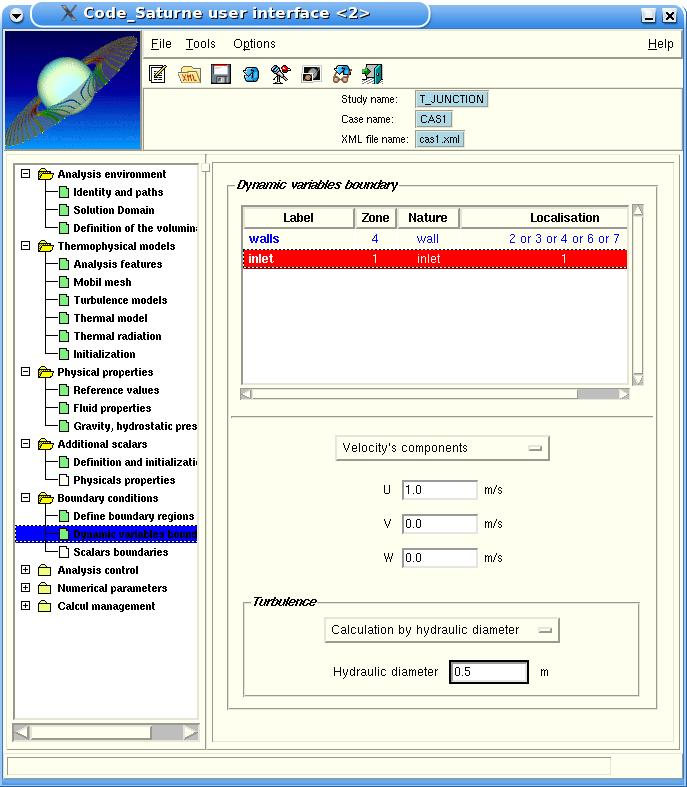
\includegraphics[width=12cm]{\repgraphics/c1_capture27.jpg} 
\caption{Dynamic variables boundary: inlet}
\label{fig27_e1}
\end{center}
\end{figure}


\clearpage
As for the wall boundary zone, the only specification the user might have to
give is when the wall is sliding. In this case, the walls are fixed so the
option is left ``off''.

Note that if one of the walls had been sliding, it would have been necessary to
isolate the corresponding boundary faces in a specific boundary region.

\begin{figure}[ht]
\begin{center}
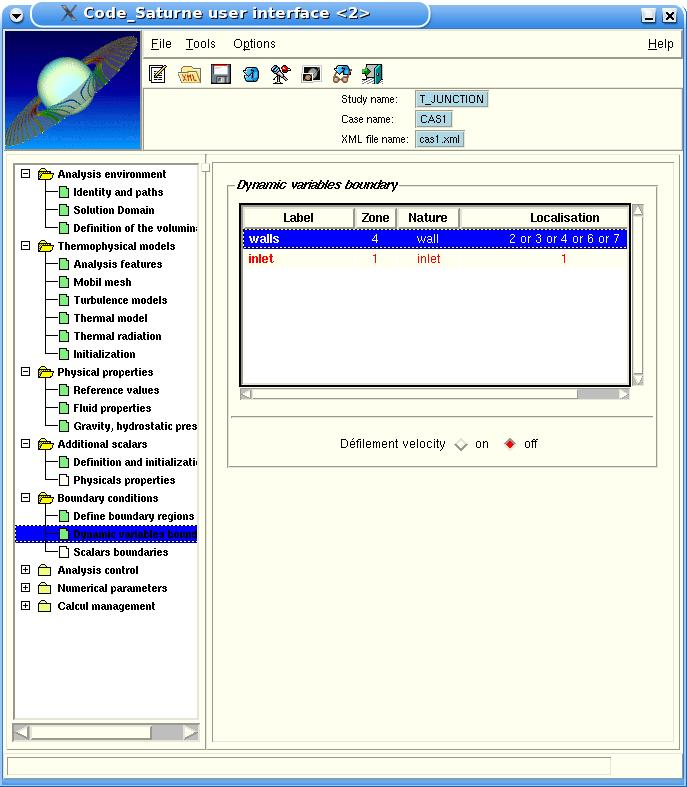
\includegraphics[width=12cm]{\repgraphics/c1_capture28.jpg} 
\caption{Dynamic variables boundary: walls}
\label{fig28_e1}
\end{center}
\end{figure} 


\clearpage
click on the item {\itshape Scalars boundaries} to set the boundary conditions
on the scalar. Only inlets, outlets and walls are concerned.

For the walls, three conditions are available:\\
\hspace*{1cm}$\bullet\ ${\itshape Dirichlet}\\
\hspace*{1cm}$\bullet\ ${\itshape Neumann}\\
\hspace*{1cm}$\bullet\ ${\itshape Exchange Coefficient}

For the outlet, only Dirichlet and Neumann conditions are available, but they are
taken into account only when the flow re-enters from the oultet. Otherwise,
homogeneous Neumann is considered by \CS.

For the inlets, only a Dirichlet condition is available.

\begin{figure}[ht]
\begin{center}
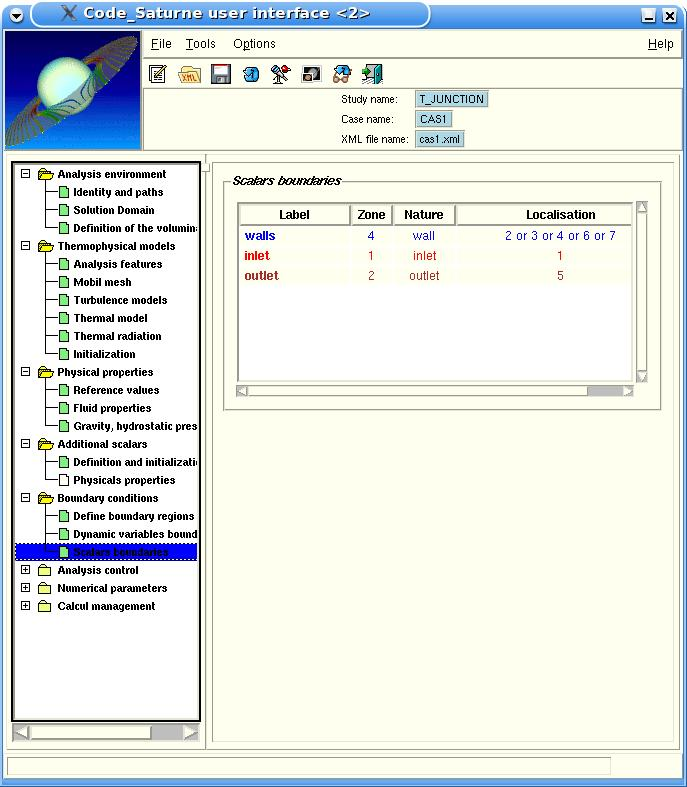
\includegraphics[width=12cm]{\repgraphics/c1_capture29.jpg} 
\caption{Scalars boundaries}
\label{fig29_e1}
\end{center}
\end{figure}


\clearpage 
In this case all walls are adiabatic. So the boundary condition for the
temperature will be a {\itshape Neumann} condition with 0 for the value. 
\begin{figure}[ht]
\begin{center}
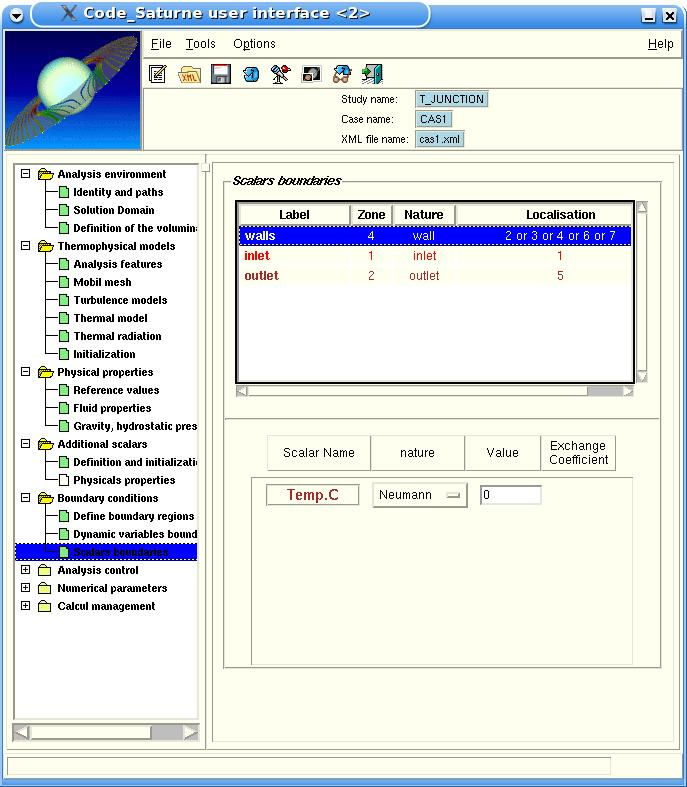
\includegraphics[width=12cm]{\repgraphics/c1_capture30.jpg} 
\caption{Scalars boundaries: walls}
\label{fig30_e1}
\end{center}
\end{figure}


\clearpage
Click on {\itshape inlet} to choose the temperature inlet
value. Here this value is 300\degresC. 
The default value is left for the outlet.

\begin{figure}[ht]
\begin{center}
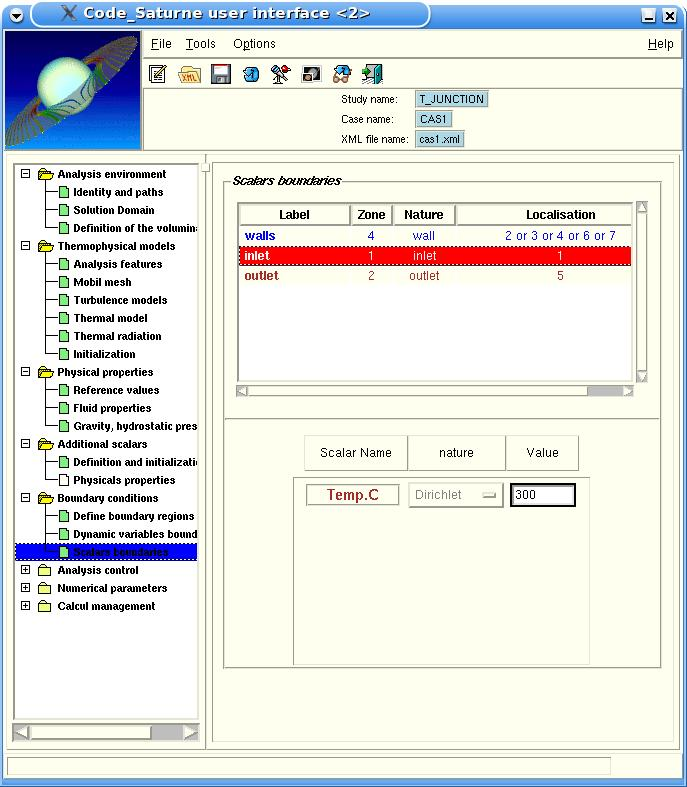
\includegraphics[width=12cm]{\repgraphics/c1_capture31.jpg} 
\caption{Scalars boundaries: inlet}
\label{fig31_e1}
\end{center}
\end{figure}


\clearpage
The calculation parameters need then to be specified, under the header {\itshape
Analysis control}.

Go to the item {\itshape Steady management} to specify the number of iterations,
30 in this case. The default value of the relaxation
coefficient will be kept and  the
{\itshape Option zero iteration} will not be activated. 

\begin{figure}[ht]
\begin{center}
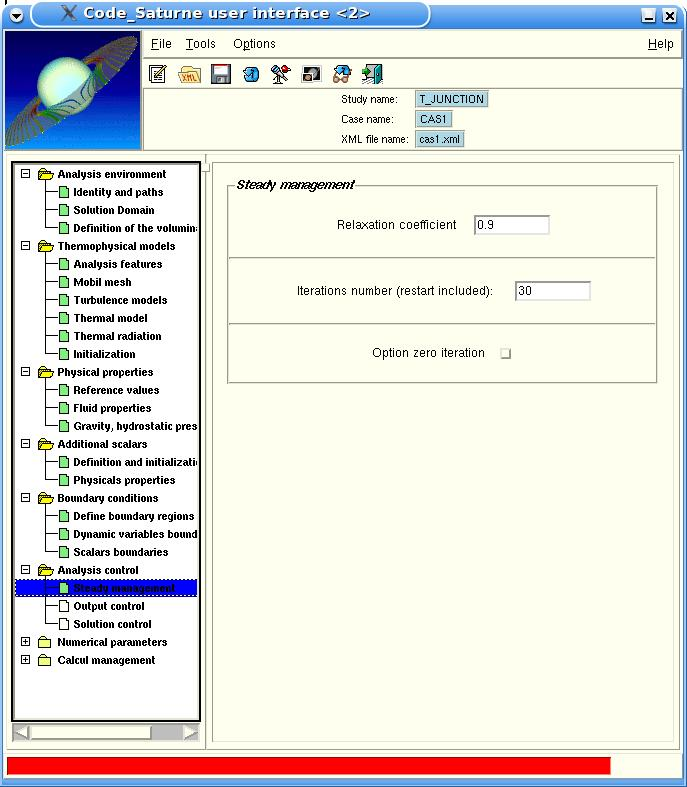
\includegraphics[width=12cm]{\repgraphics/c1_capture32.jpg} 
\caption{Steady flow management}
\label{fig32_e1}
\end{center}
\end{figure}


\clearpage
Click on the item {\itshape Output control} to change the frequency for the
printing of information in the output listing. 
The options are:\\
\hspace*{1cm}$\bullet\ ${\itshape No output}\\
\hspace*{1cm}$\bullet\ ${\itshape Output listing at each time step}\\
\hspace*{1cm}$\bullet\ ${\itshape Output at each 'n' time step} (the value of
'n' must then be specified)\\
Here and in most cases, the second option should be chosen.

\begin{figure}[ht]
\begin{center}
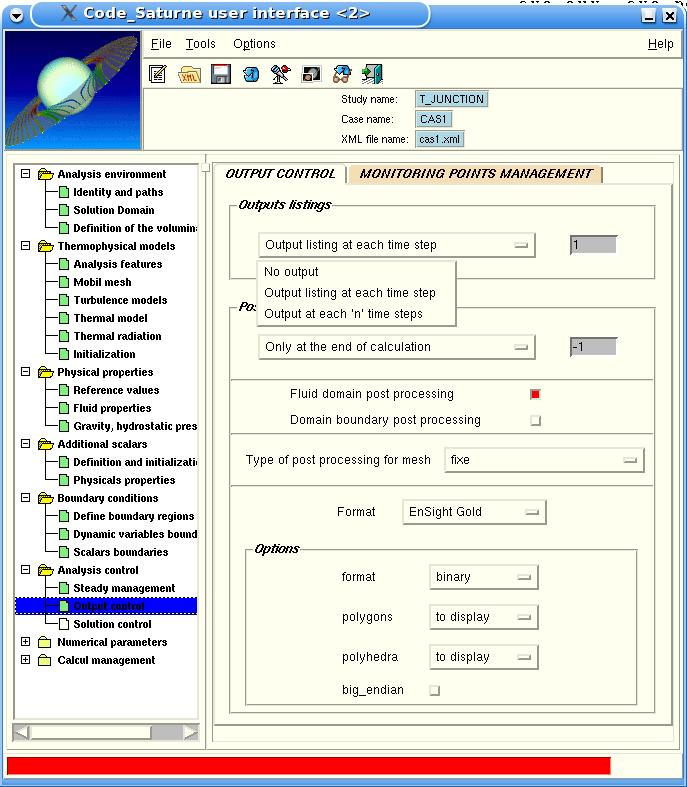
\includegraphics[width=12cm]{\repgraphics/c1_capture33.jpg} 
\caption{Output control: output listing}
\label{fig33_e1}
\end{center}
\end{figure}


\clearpage
For the post-processing (by default EnSight format files), there are two options:\\
\hspace*{1cm}$\bullet\ ${\itshape Only at the end of calculation}\\
\hspace*{1cm}$\bullet\ ${\itshape Chronologics at each 'n' time steps}

In this case, we are interested in the evolution of the variables during the
calculation, so the second option is chosen with a value of 1 for 'n'.

\begin{figure}[ht]
\begin{center}
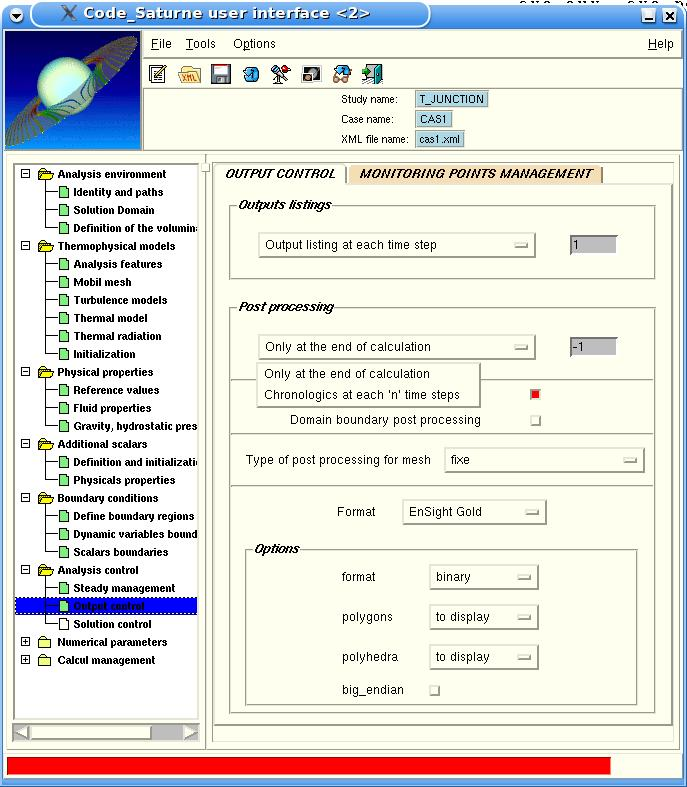
\includegraphics[width=12cm]{\repgraphics/c1_capture34.jpg} 
\caption{Output control: post-processing}
\label{fig34_e1}
\end{center}
\end{figure}


\clearpage
The other options are kept to their default value.

\begin{figure}[ht]
\begin{center}
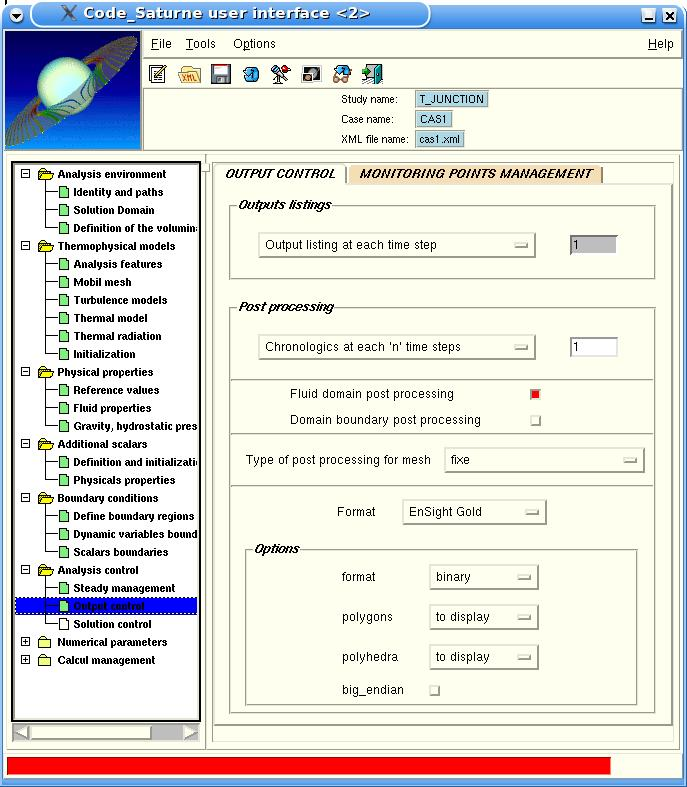
\includegraphics[width=12cm]{\repgraphics/c1_capture35.jpg} 
\caption{Output control}
\label{fig35_e1}
\end{center}
\end{figure}
 
The {\itshape Monitoring points management} tab allows to define specific points
in the domain (monitoring probes) where the time evolution of the different
variables will be stored in historic files. In this case no monitoring points
are defined.


\clearpage
The item {\itshape Solution control} allows to specify which variable will
appear in the output listing, in the post-processing files or on the
monitoring probes. In this case, the default value is kept, where every variable
is activated. 


\begin{figure}[ht]
\begin{center}
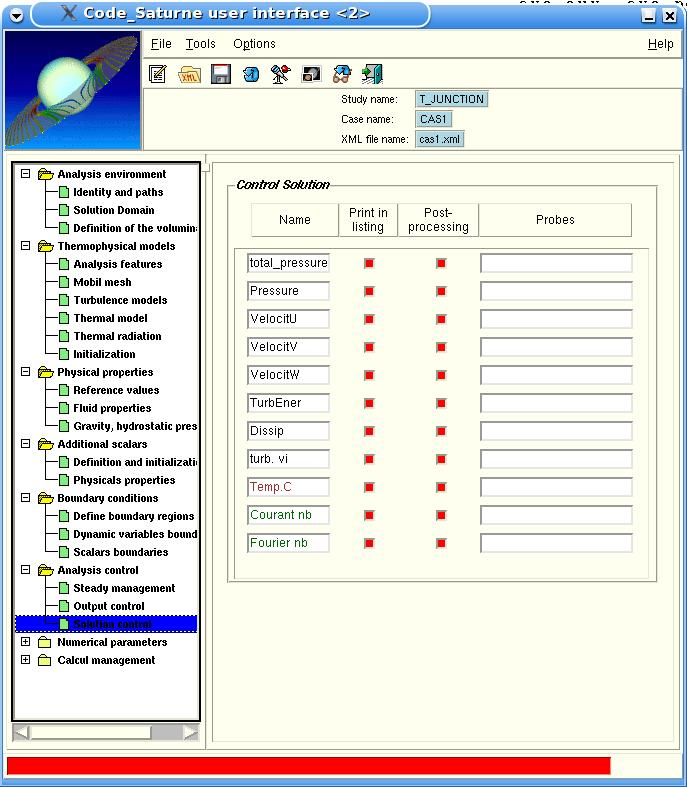
\includegraphics[width=12cm]{\repgraphics/c1_capture36.jpg} 
\caption{Solution control}
\label{fig36_e1}
\end{center}
\end{figure}


\clearpage
The heading {\itshape Numerical parameters} allows to change different more
advanced numerical parameters. In this case none of them should be changed from
their default value.

\begin{figure}[!h]
\begin{center}
\begin{tabular}{c}
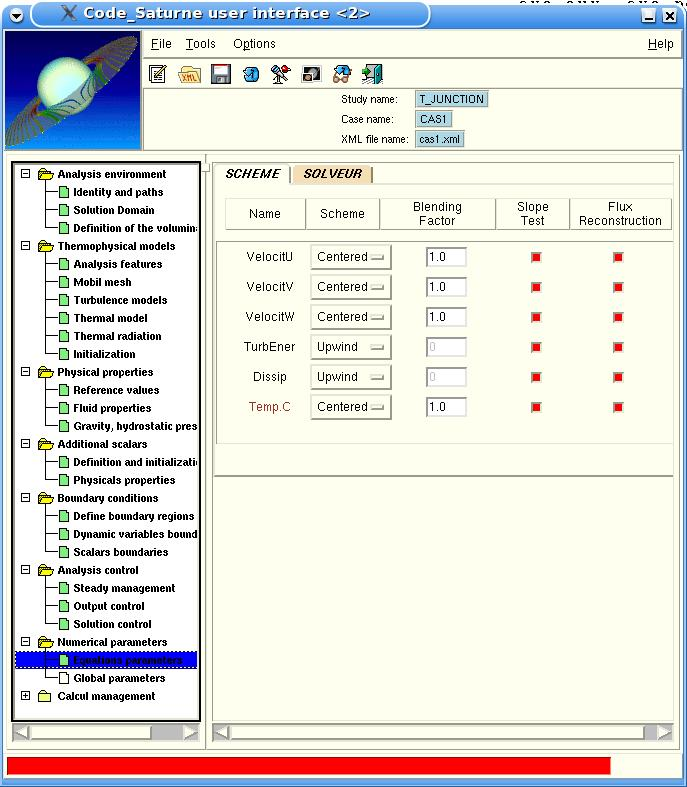
\includegraphics[width=9cm]{\repgraphics/c1_capture37.jpg}\\
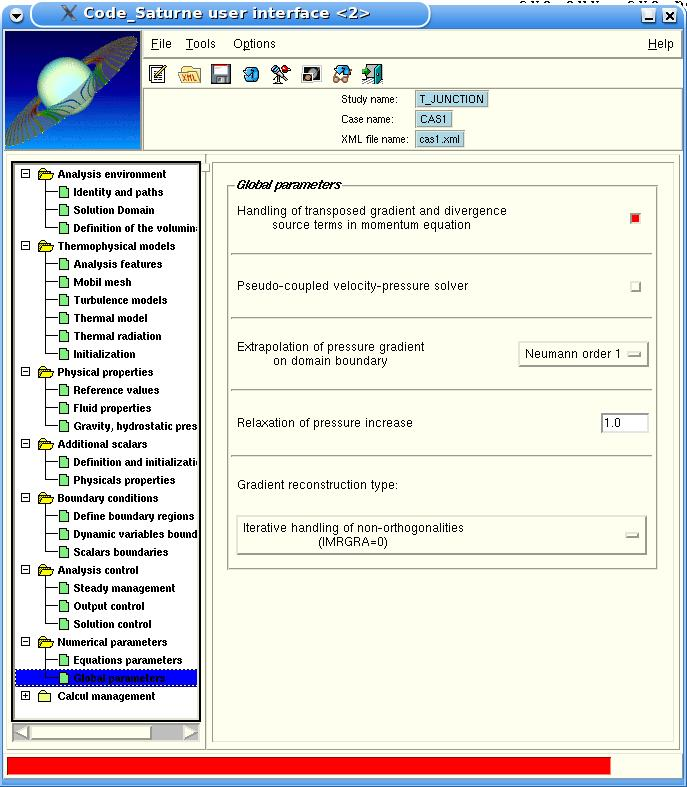
\includegraphics[width=9cm]{\repgraphics/c1_capture38.jpg} 
\end{tabular}
\caption{Numerical parameters}
\label{fig3738_e1}
\end{center}
\end{figure}


\clearpage
When using Fortran routines, it is sometimes useful to allocate pre-defined user
arrays, that are present in every sub-routine. This allocation can be specified
in the {\itshape User arrays} item, under the {\itshape Calculation management}
heading. It is not the case in the present calculation.

\begin{figure}[ht]
\begin{center}
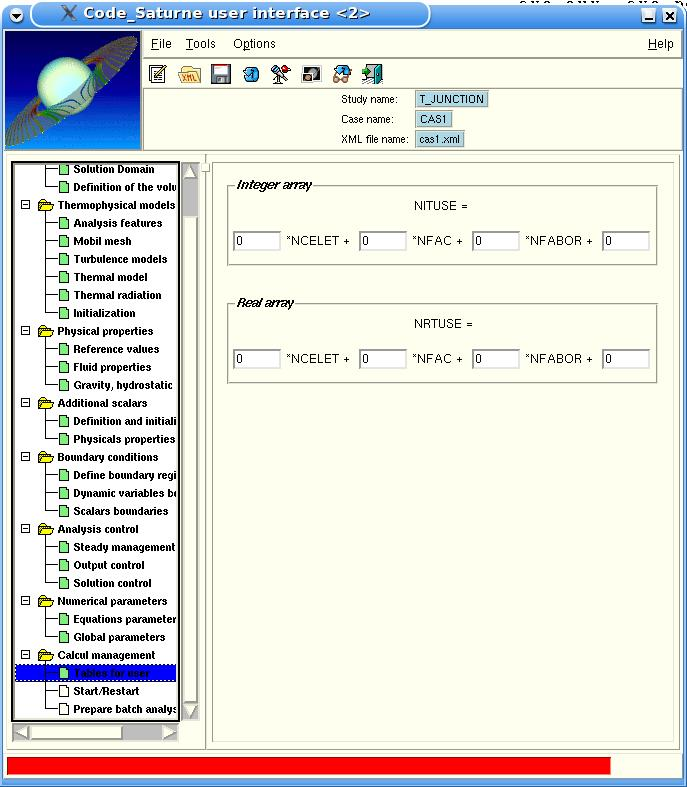
\includegraphics[width=12cm]{\repgraphics/c1_capture39.jpg} 
\caption{User arrays}
\label{fig39_e1}
\end{center}
\end{figure}


\clearpage
The item {\itshape Start/Restart} allows to start a new calculation from the
results of a former one. It is not the case in the present calculation so
nothing has to be modified.

\begin{figure}[ht]
\begin{center}
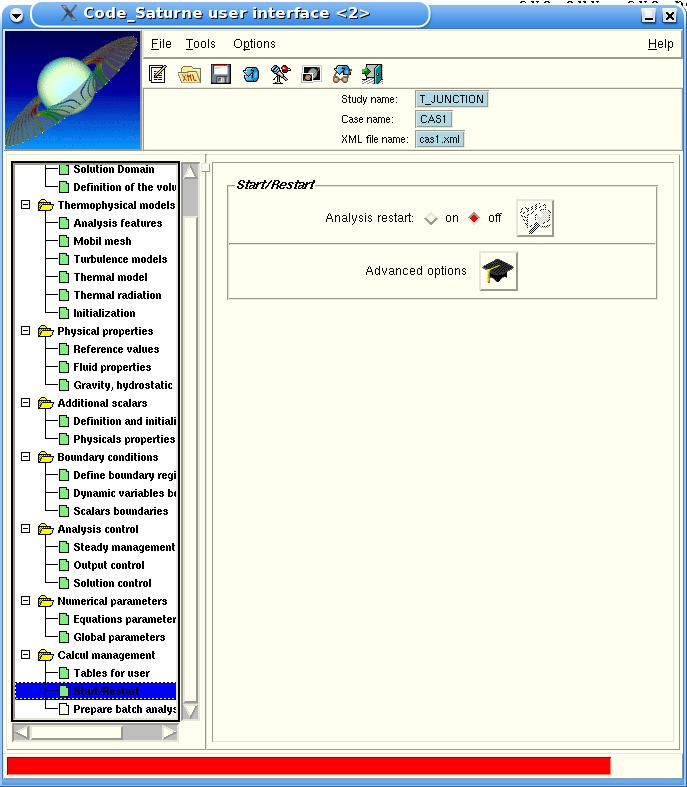
\includegraphics[width=12cm]{\repgraphics/c1_capture40.jpg} 
\caption{Start/Restart}
\label{fig40_e1}
\end{center}
\end{figure}


\clearpage
The final item, {\itshape Prepare batch analysis}, is used to prepare the launch
script and, on certain architectures, launch the calculation.

Calculations can be launched from the Graphical Interface in interactive mode
({\itshape Workstation}) or in a PBS batch queue ({\itshape Management of chart
PBS}). In this simple case, choose the Workstation.

\begin{figure}[ht]
\begin{center}
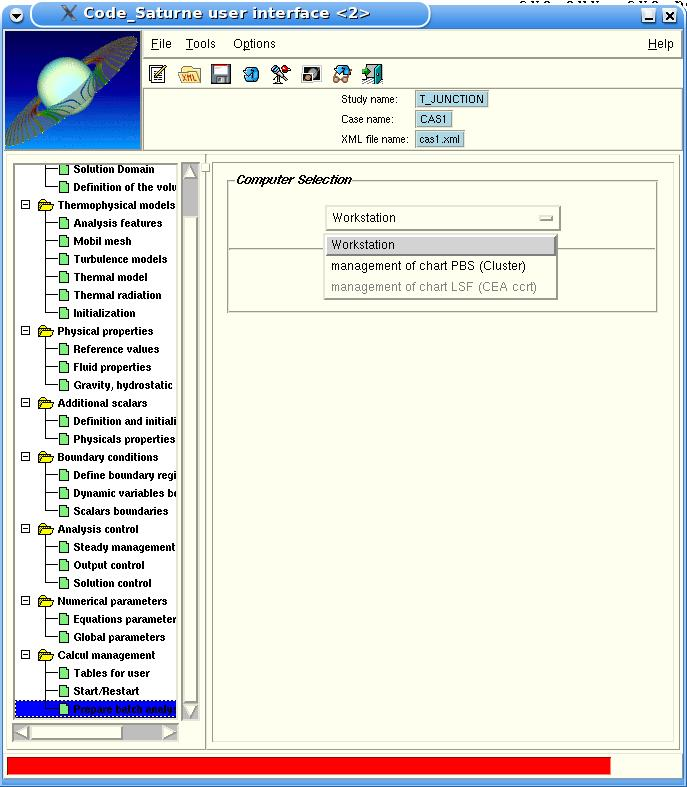
\includegraphics[width=12cm]{\repgraphics/c1_capture41.jpg} 
\caption{Prepare batch analysis: Computer selection}
\label{fig41_e1}
\end{center}
\end{figure}


\clearpage
Click on the icon to {\itshape Select the batch script file} to select the
launch script. The default launch script is named {\itshape lance} and is
situated in the SCRIPTS directory. Select it and click on {\itshape Open}.

Remember to save the Xml file before opening the launch script.

\begin{figure}[ht]
\begin{center}
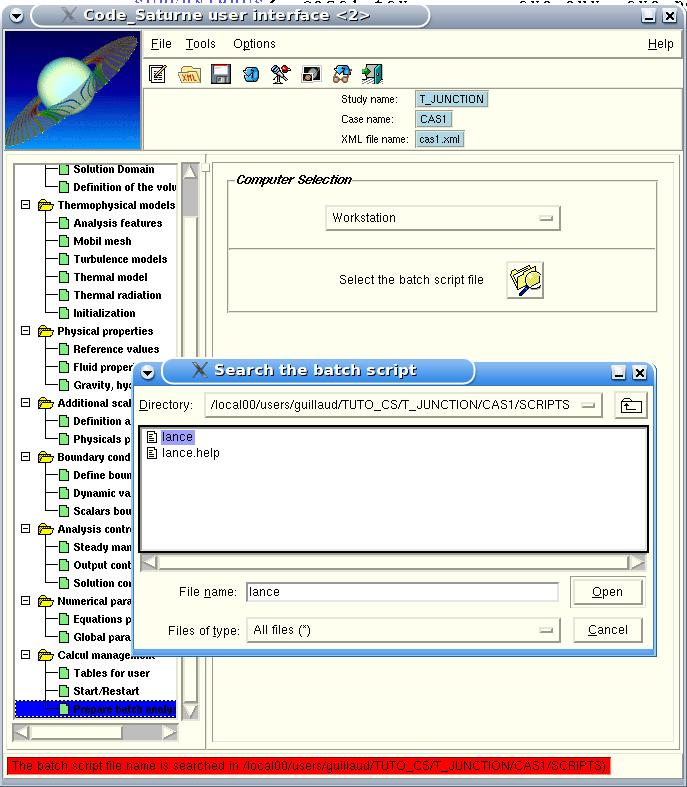
\includegraphics[width=12cm]{\repgraphics/c1_capture42.jpg} 
\caption{Prepare batch analysis: Batch script file selection}
\label{fig42_e1}
\end{center}
\end{figure}


\clearpage
When the script is selected, new options will appear. They allow to give the
memory size for the calculation. It is the size of the integer and real arrays
that will be used to store most of the variables in the Fortran parts of \CS.
It is dependent on the number of cells in the mesh. In parallel mode, it depends
on the number of cells treated by each processor, and not the total number of
cells. For this simple case, the default values are appropriate.

On this calculation, the number of processors used will be left to 1.

When launching a calculation, a temporary directory is created on the machine,
where the script copies and creates temporary files and from where the \CS\
executable is launched. Should some user routines read or write case-specific
files, they must be copied in the temporary directory, or from the temporary
directory into the RESU directory. The {\itshape User files} icon allows the
user to specify user data files (in the DATA directory) or user result files,
that will then be copied automatically to or from the temporary directory.
In this example, no user file is needed.

Finally, the {\itshape Advanced options} icon allows to change some more
advanced parameters that will not be needed in this simple case.

Eventually, save the Xml file and execute it by clicking on
{\itshape \CS\ batch running}. The results will be copied in the RESU
directory.

\begin{figure}[ht]
\begin{center}
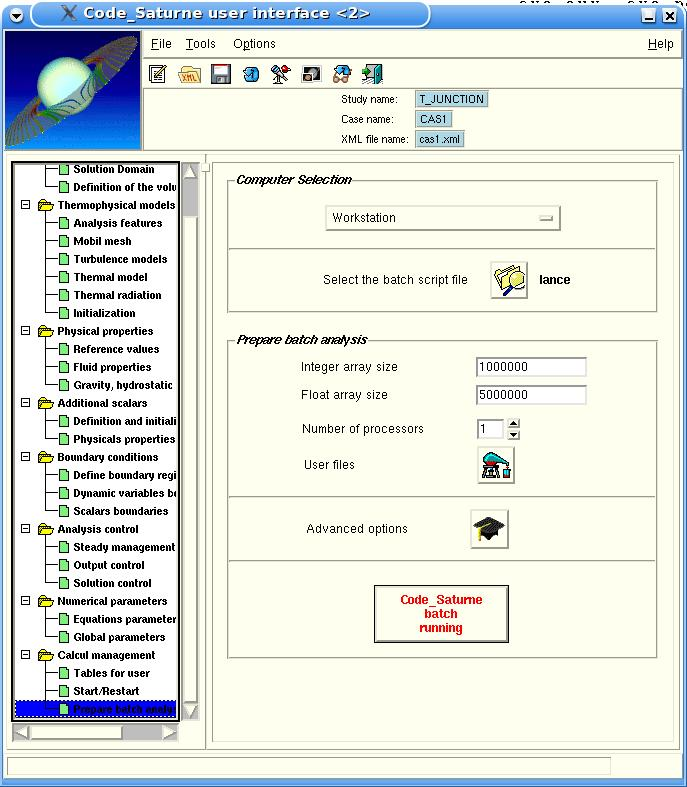
\includegraphics[width=12cm]{\repgraphics/c1_capture43.jpg} 
\caption{Prepare batch analysis: Execution}
\label{fig43_e1}
\end{center}
\end{figure}


